\chapter*{Preface}

\section*{The network machine learning earthquake}

In the early 1990s, a Computer Science PhD student at Stanford University decided to focus on the interconnectedness of the world wide web, which has since become the backbone of the modern internet.

With the assistance of a colleague, Sergey Brin, Page determined that the complicated set of links between documents on the world wide web could best be understood as a large \textit{network}, in which the objects on the world wide web (primarily documents) were interconnected through a series of links. These links allow one to ``jump'' from one document to the next in a sequential fashion. The number of documents which linked to a reference document, Page and Brin theorized, gave some notion of the ``popularity'', or the \textit{page rank}. Being out-of-the-box thinkers, Page and Brin took this idea and combined it with many other strategies: in particular, they developed a query system which allowed a sentence to be parsed into keywords, and then they developed an indexing system which mapped these keywords to the pages with the highest pagerank. After publishing several papers and getting a number of other computer scientists involved in the project, Page and Brin developed a prototype of the Google search Engine in 1998, and shortly thereafter, founded Google Inc. From there, the rest is history.

Fast forward, and networks have become a dominant data structure with which to understand many of the concepts of every day life. Social networks have led to a new rise in the interconnectedness of people, led by massive multi-billion dollar corporations such as Facebook, Twitter, Linkedin, Instagram, Douyin (TikTok), and WeChat. The economy forms a global interconnected trade network, wherein companies and countries interact with one another for daily commercial benefits. The Earth's food chain forms an ecological network, in which plants and animals fight for survival in an unforgiving world. Neurons of the brain form an interconnected web of axons and synapses, together producing unique aspects about what make you really you. 

\section*{Network Machine learning in your projects}

Recent developments in network science have produced new strategies with which you can hope to understand and derive insights from this pervasive way to understand the world. 

Perhaps you're a researcher and you want to expose shadowy financial networks and corporate fraud? Or create a network framework for measuring teamwork in healthcare? Maybe you're interested in ecological releationships between different animals, or maybe you want to model communities of neurons in the brain?

Or maybe you're a data scientist and your company has tons of data (user logs, financial data, production data, machine sensor data, hotline stats, HR reports, etc.), and more than likely you could view the data as a network and unearth some hidden gems of knowledge if you just knew where to look?

Whatever the reason, you have decided to explore and exploit networks and implement their analysis in your projects. Great idea!

\subsection*{Objective and approach}
This book assumes you know next to nothing about how you can explore and exploit network data. Its goal is to give you the concepts, the intuitions, and the tools you need to allow you to incorporate techniques from statistical learning and data science with network data, as shown in Figure \ref{fig:this_book}.

Whoever you are, we think you'll find a lot of things that are useful and interesting in this book.


\begin{figure}[h]
    \centering
    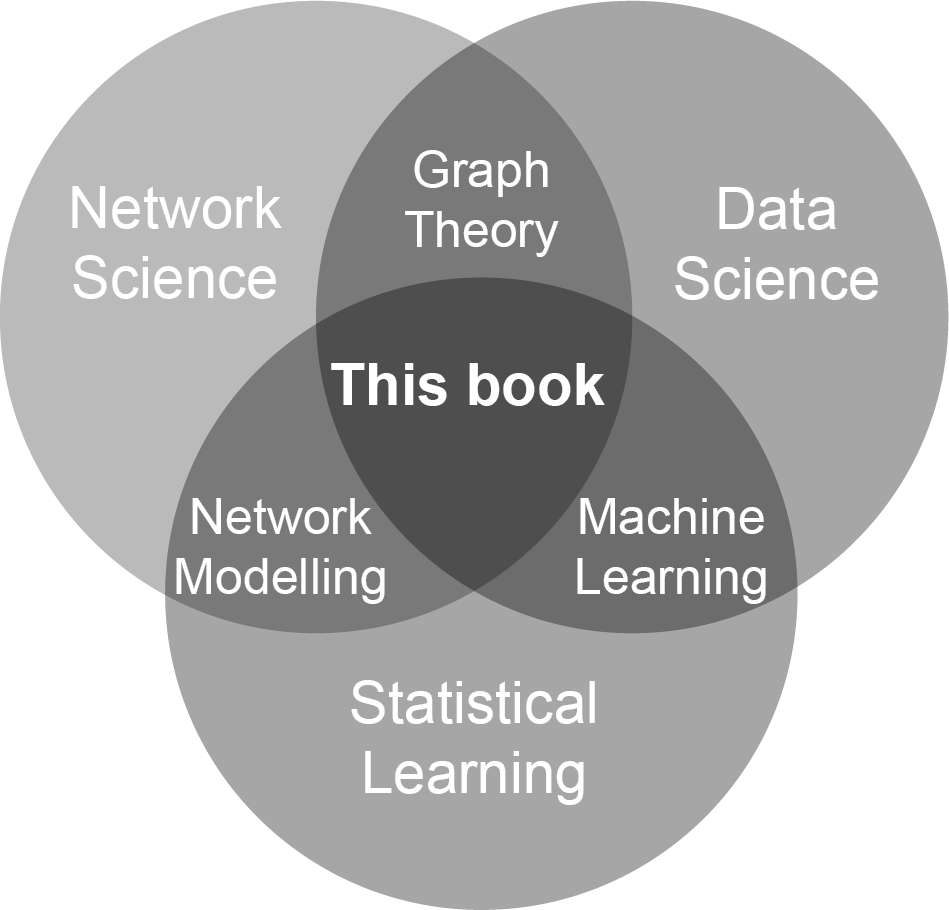
\includegraphics{Images/this_book.png}
    \caption[Venn diagram of network machine learning]{Broadly, we think that the techniques developed and described in this book fall somewhere in the middle of this Venn Diagram.}
    \label{fig:this_book}
\end{figure}

We'll cover the fundamentals of network machine learning, focusing on developing intuition on networks with relevant \texttt{python} tutorials. By the end of this book, you will be able to utilize efficient and easy-to-use tools available for performing analyses on networks. You will also have a whole new range of techniques in your toolbox, such as representations, theory, and algorithms for networks.

We'll show how to do this using production-ready \texttt{python} frameworks:
\begin{enumerate}
    \item \texttt{numpy} \cite{numpy} and \texttt{scipy} \cite{scipy} are used for scientific programming. They give you access to array objects, which are the main way we'll represent networks computationally.
    \item \texttt{scikit-learn} \cite{sklearn} is very easy-to-use, yet it implements many machine learning algorithms efficiently, so it makes a great entry point for downstream analysis of networks.
    \item \texttt{graspologic} \cite{graspologic} and \texttt{networkx} \cite{networkx} are an open-source Python packages which gives you utilities and algorithms for doing analyses on network-valued data.
\end{enumerate}

We focus on developing an intuitive understanding of networks with concrete working examples and a bit of theory. While you can read this book without picking up your laptop, we highly recommend you experiment with the code examples available interspersed throughout the book.

There are many languages and software packages that are extremely useful for network data. When writing this book, we were faced with numerous design choices, and unfortunately it is not feasible to write the entire textbook with tools for every possible language or package for network analysis. There are numerous packages and built-in utilities in \texttt{matlab}, and \texttt{R} has the \texttt{igraph} \cite{csardi2006} package which provides complementary functionality to many of the techniques we discuss herein.

If you are unfamiliar with \texttt{python} but are familiar with another language, we do not think you will find this to be a substantial hurdle (and you might even come out of it with a new programming language skill!). 

\section*{Prerequisites}

Because network science uses a lot of linear algebra, requiring a bit of linear algebra knowledge is unavoidable. We expect you have some familiarity with matrices and the basic operations you can do with them: multiplication, addition, and so on.

If you want to best understand the concepts of this book, we think it would be valuable for you to come in with some background in machine learning. Much of the content will very related to a particular sub-domain of machine learning known as \textit{statistical learning}. This area of research focuses on incorporating statistics with machine learning to better understand and analyze machine learning algorithms. We will assume that you are loosely familiar with probability and statistics (you know what it means for something to be random), but we won't delve too deep into the weeds.

You should also probably have some background in programming -- we'll mainly be using \texttt{python} to build and explore our networks. If you don't have too much of a Python or math background, don't worry -- we'll link some resources to give you a head start.

Another tool we will use, \texttt{jupyter}, is a great tool to have in your toolbox and it's easy to learn. We'll also link some resources for you if you are not familiar with Python's scientific libraries, and we provide a full scientific container pre-loaded with a full programming environment already set up for you in one-click via \texttt{docker} \cite{docker}. 

If you care about what's under the hood, we have appendices which isolate the theoretical underpinnings of the techniques developed herein -- you should have a reasonable understanding of college-level math, such as calculus, linear algebra, probability, and statistics for these sections.

\section*{Roadmap}

This book is organized into four parts.

\begin{itemize}[leftmargin=1cm]
    \item [Part \ref{p:found}] Foundations gives you a brief overview of the kinds of things you'll be doing in this book, and shows you how to solve a network machine learning problem from start to finish. It covers the following topics:
    \begin{itemize}
        \item What a network is and where you can find network data
        \item Many the reasons why we study network data
        \item Examples of ways you could apply network machine learning to your own projects
        \item An overview of the types of problems network machine learning is good at dealing with
        \item Exploring a real network machine learning dataset, to get a broad understanding of what you might be able to learn
    \end{itemize}
    \item [Part \ref{p:rep}] Representations is all about how we can conceptualize networks intuitively, and what we can do with differents ways to represent and conceptualize them. It covers the following topics:
    \begin{itemize}
        \item The various useful properties different types of networks have
        \item Types of network representations and why they're useful
        \item Ways you can represent individual or groups of networks
        \item How to represent networks or groups of networks as tabular data
        \item How to incorporate additional information (attributions) to networks
    \end{itemize}
    \item [Part \ref{p:app}] Applications is about using the representations from Part \ref{p:rep} to explore and exploit your networks for downstream tasks. It covers the following topics:
    \begin{itemize}
        \item Figuring out if communities in your networks are different from each other
        \item Selecting a reasonable model to represent your data
        \item Finding nodes, edges, or communities in your networks that are interesting
        \item Finding time points which are anomalies in a network that is evolving over time
        \item What to do when you have new data after you've already trained a network model
        \item How hypothesis testing works with networks
        \item Figuring out which nodes are the most similar in a pair of networks
    \end{itemize}
    \item [Part \ref{p:next}] Next Steps discusses concepts that don't directly tie into the story we hope to tell, but we believe they are extremely important ideas to be aware of and introduced to, and we believe that we can help situate you with these concepts so that you can learn more about them on your own. They are:
    \begin{itemize}
        \item Graph neural networks
        \item Diffusion methods for networks
        \item Network sparsity
        \item a path forward for you to continue your journey with network machine learning
    \end{itemize}
\end{itemize}
The appendices provide an brief overview of what we consider to be higher-level concepts. In the interest of keeping this book approachable, the main content of the work has, admittedly, left out many technical details and considerations that might be very useful for readers farther along in their journey through math and statistics. You will find these details in here.

\section*{Other resources}

Many resources exist which will help you greatly with the content of this book. 

If you don't have any background in machine learning quite yet, our favorite starting point is Aur\'elian G\'eron's excellent work \cite{Geron2017Mar}. We would recommend starting with an introduction to machine learning \textit{prior to} focusing on this book, because many of the concepts and ideas of this text will make more sense coming in with a machine learning background, however brief. The core ideas you should remember are the types of machine learning problems, some of the more common algorithms and techniques for machine learning (\texttt{K-Means}, testing, and validation each come up a few times), and the basic data structures used for machine learning.

To our knowledge, there are no other books which explicitly focus on network machine learning for single and multiple network problems just yet, and moreover, there are also none that do this with a programming component. If you want some more exposure to networks in general, we would recommend the following works:
\begin{enumerate}
    \item ``Network Science'' \cite{Barabasi2016Aug}, which provides an approachable and well-grounded introduction to network science.
    \item ``Networks'' \cite{Newman2018Sep}, which provides an expansive glance at the mathematics of networks and network models.
    \item ``Python for Graph and Network Analysis''\cite{AlTaie2017}, which presents network analysis techniques in \texttt{python}.
    \item ``Network Analysis'' \cite{Brandes2005}, which focuses on the development of the network data structure and summary statistics for networks.
    \item ``A User's Guide to Network Analysis in \texttt{R}'' \cite{Luke2015}, which provides a hands-on introduction to network analytics techniques in the \texttt{R} programming language.
    \item ``Statistical Analysis of Network Data'' \cite{Kolaczyk2009}, which presents statistical models and methods for network science.
\end{enumerate}

If you haven't seen linear algebra in a while, we would recommend that you start with the book ``Numerical Linear Algebra'' \citep{Trefethen1997}, by Trefethan and Bau. The first 4 lectures succinctly and effectively summarize all of the properties of matrices that we will need for this book. You will also want to have some exposure to basic statistics and statistical inference; if you can read and understand the wikipedia summaries (at the top of the page) on ``random variable'', ``normal distribution'', and ``bernoulli distribution'', we think that you will have plenty of statistical background to make it through this book. 

If you are looking for a more comprehensive overview, a good introduction is \citep{Casella2001Jun} by Casella and Berger, and a good refresher is \cite{Bickel2006May} by Bickel and Doksum. It may also be helpful to be explicitly introduced to statistical learning; our favorite is \citep{James2021Jul}, by Jones, Witten, Hastie, and Tibshirani.

\begin{comment}
\section*{Material we won't cover}

The network data structure has quickly become a go-to across many domains of science and industry. One application of networks is particularly appealing: networks can be used to succinctly conceptualize and visualize underlying relationships that exist outside of just network-valued data. One of the most prominent applications of this concept uses machinery known as a \textit{Directed Acyclic Graph} (or DAG) to conceptualize the ``flow'' between different elements in an underlying system. Since graph is just another word for network, this concept is inherently rooted in networks. 
\end{comment}

\section*{Conventions used in this book}

The following conventions are used in this book:

\begin{itemize}
    \item \emph{Italics}: indicates emphasis behind a term or exclamation. Also often used when terms have not yet been defined, but a definition is upcoming.
    \item \textbf{Bold face}: indicates a definition for a term or concept.
    \item \texttt{Unicode block}: used to indicate the name of an algorithm, function names, package names, programmatic text elements, and related concepts.
\end{itemize}

\begin{floatingbox}[h]
\caption{Remarks}
Used to indicate ideas that are directly relevant or supplementary to the content of the book, but are not essential for understanding the main concepts of a section or paragraph.
\label{fb}
\end{floatingbox}

\subsection*{Code examples}

The entirety of this book has been compiled using \texttt{jupyter} notebooks, integrated through the \texttt{jupyter-book} framework. The book is currently hosted on github at \texttt{github.com/neurodata/graph-stats-book}, and the build log for the text can be found at \texttt{github.com/neurodata/graph-stats-book/actions}. You can find every section notebook, and every command which was used to prepare the environment in which the corresponding textbook pages were executed, using those two links. 

All of the code used to prepare simulations or algorithms are contained within this book. For example, a python code block, and its corresponding expected output, will look like this:
\begin{lstlisting}[style=python]
def howdy_world():
    # A function to print informative text.
    print("Howdy world!")
howdy_world()
# Hello world!
\end{lstlisting}

When discussing how to set up your initial environment, we'll occassionally demonstrate \texttt{bash} commands that should be used directly from a terminal session. If you have Mac or Linux operating systems, you can get to these directly using the \texttt{terminal} utility, which should come with your computer pre-installed. If you have a Window's operating system, things are a little bit more complicated, but we have some instructions for you in Chapter \ref{sec:ch2}.

Bash code blocks can be identified by code blocks that start with a \texttt{\$}, and will look like this:

\begin{lstlisting}[style=bash]
$ echo "these is a bash demo"
this is a bash demo
\end{lstlisting}


Throughout this book, we will focus a lot of attention on visualizations and plotting, the code for which can quickly become extremely cumbersome. For all programmatically generated figures, we will show you how to generate the figure first with explicit code, and then will assume that you will be able to generate these plots on your own later on. That said, the code to recreate all plots can be found online, at \texttt{docs.neurodata.io/graph-stats-book}. Simply page to the appropriate section of the book, and identify the appropriate plot that you want to recreate. 

\paragraph*{A disclaimer about the impact of randomness}

In most of our examples, we are going to use simulations and approaches which inherently involve randomness. Running the same piece of code twice, you will probably not get the same result. The reason that we do this is two-fold:
\begin{enumerate}
    \item Using simulations will allow you to modify, manipulate, and ``play with'' the algorithms and approaches so that you can build insight. We are hoping that this book will be ``hands-on'' on your end: we \textit{want} you to try to vary around the networks that you are using as you go, so that you can challenge your intuition and use what you observe to solidify or modify your intuition accordingly. This has the caveat that every simulation run will produce a slightly different answer, and your plots might not match up with the plots that we produce exactly.
    \item Many algorithms that deal with networks use some hints of randomness to achieve solutions which are either faster or numerically superior to solutions that do not use randomness. In getting you accustomed to working with network data using approaches that are relevant in the field, we cannot ignore these techniques. Running the same algorithm on the same network twice might produce slightly different results.
\end{enumerate}

That said, the broad implications of each code segment on your machine should produce a similar (but perhaps not identical) conclusion to what we reach in our plots. If a particular technique will be problematic, we will hard-code 


\subsection*{Using code examples, citing the book, and reaching out with feedback}

This book is intended to teach you how to develop code for network machine learning. In general, we are providing this code for you: it is intended that you will borrow and repurpose the code and techniques we describe in your programs and documentation. If you are using a few brief snippets from our book for your work, feel free with proper attribution to our citation (below). If you want to write a program that borrows some code, feel free without permission. If you intend to sell or financially profit directly from code we provide in this book, you need to request permission.

To cite our textbook, you can use the following citation: 

Eric W. Bridgeford, Alexander R. Loftus, and Joshua T. Vogelstein. \emph{Hands-on Network Machine Learning with Scikit-Learn and Graspologic}. Cambridge University Press.

To request permissions, provide us with feedback about our in-progress draft, or even just to say hi and let us know what network machine learning concepts you want to see us discuss, feel free to reach out to the authors directly. You can reach out to us at \texttt{ericwb95@gmail.com}.

\subsection*{About the authors}

\textbf{Eric W. Bridgeford} is a Ph.D. student in the Department of Biostatistics at Johns Hopkins University. Eric’s background includes Computer Science and Biomedical Engineering, and he is an avid contributor of packages to \texttt{CRAN} and \texttt{pypi} for nonparametric hypothesis testing. Eric's research focuses on general approaches bridging causal inference with high-dimensional statistical methods to learn about sources of variability in complex data such as networks. He was a core contributor to the backbone of the \texttt{graspologic} package. Eric authored most of the content, examples, code segments, docker container, and the supplementary \texttt{graphbook-code} package used within the book.

\noindent\textbf{Alexander R. Loftus} was a master’s student at Johns Hopkins University in the Department of Biomedical Engineering, with an undergraduate degree in neuroscience. He has worked on implementing network spectral embedding and clustering algorithms in Python, and helped develop an MRI pipeline to produce brain networks from diffusion MRI data. Alex played a valuable role with visualization and data architecting of the \texttt{graphbook-code} package, and helped construct outlines and drafts for several sections of the book. Alex has been extremely critical with feedback throughout the writing process.

\noindent\textbf{Joshua T. Vogelstein, Ph.D.} is an Associate Professor in the Department of Biomedical Engineering at Johns Hopkins University, with joint appointments in Applied Mathematics and Statistics, Computer Science, Electrical and Computer Engineering, Neuroscience, and Biostatistics. His research focuses on the statistics of networks in brain science (connectomes). Josh, along with his lab and collaborators, have developed many leading computational algorithms and libraries to perform statistical analysis on networks, which serve as the philosophical foundation upon which this book rests. 

\paragraph{Section Contributors}

\textbf{Jes{\'u}s Daniel Arroyo, Ph.D.} is an Assistant Professor in the Department of Statistics at Texas A\&M University. He focuses on the theoretical underpinnings of statistical network analysis, machine learning, and high-dimensional data analysis, including topics such as spectral graph inference, dimensionality reduction, convex optimization, and graph matching. Jes\'us tends to focus on the applications of his work to neuroimaging data in statistical connectomics. Jes\'us played a key role as a proofreader for a number of sections in the book, and helped us draft the appendix outlining the theory behind network machine learning strategies.

\noindent\textbf{Ali Saad-Eldin} is a software engineer at Amazon. As a masters student at Johns Hopkins University in Applied Mathematics and Statistics, Ali focused his attention on optimization techniques for solving problems in graph analysis. He was a core contributor to the \texttt{graspologic} package and developed the submodule for graph matching. Ali helped to write the section on graph matching.

\noindent\textbf{Sambit Panda} is a Ph.D. student at Johns Hopkins University in the Department of Biomedical Engineering. Sambit's work focuses on nonparametric hypothesis testing for large datasets, with applications in neuroimaging. He was a core contributor to the `hyppo` package, which is a python framework for hypothesis testing. Sambit helped to write the section on two-sample hypothesis testing.

\noindent\textbf{Jason Yim} is a Ph.D. student at Massachusetts Institute of Technology in the Department of Electrical Engineering and Computer Science (EECS), where he develops generative models for de-novo protein design. Prior to starting his PhD, Jason focused on the application of neural networks to protein folding and macular degeneration with DeepMind, a company focused on artificial intelligence that was acquired by Google in 2014. Jason helped to write the section on graph neural networks.

\section*{Acknowledgements}

First and foremost, we want to acknowledge all of the monumental contributions to science that made this book possible. We would not have been capable of producing this work without the work of our many collaborators and the greater scientific community. Academic-focused books are produced as much by the authors as they are by the many wonderful contributors that developed the works that comprise this book. Throughout each chapter of this book, we'll list out the key papers in the bibliography that you can check out that led to the insights that go into each section. You can use these papers in conjunction with the appendix (where applicable) to find more detailed and technical descriptions of the particular algorithms and techniques we describe in this book. 

Finally, we want to offer a big thanks to everybody who has been reading the book as we write. So far, this list includes our wonderful editor Lauren Cowles, as well as Dax Pryce, Ross Lawrence, Geoff Loftus, Alexandra McCoy, Olivia Taylor, and Peter Brown. Writing a large textbook is not easy, and we truly appreciate all of the gracious feedback that we have been offered throughout the writing stages as we refine this book.

\bibliographystyle{vancouver}
\bibliography{references}